\section{Dice, Bce and NQM}
\label{experiments:02.0:intro}
We decided to investigate whether it is possible to include the NQM in the training loop to improve the robustness of the model by implementing the NQM directly as a loss function or using it within the training loop. However, as seen in \autoref{experiments:01.0:Into}, it is technically possible but not very useful to use the NQM as a loss on its own. Therefore, in this section, we will focus on our attempts to implement a loss function that takes the NQM into account but not depends only on it. In \autoref{experiments:02.1:diceBce+NQM}, we will see the implementation that has worked best here, and which we have also used for most of the robustness improvement experiments (\autoref{experiments:03.0:Intro}). For completeness, the rest of this section will show some other attempts at loss functions that worked worse or not at all and that we discarded after testing them here. We also tested some other implementations not presented here, particularly those we re-tested in \autoref{experiments:03.1.x:FurtherNQMLosses}. These did not show any improvement over the DiceBceNQM loss here. They will be presented in \autoref{experiments:03.1.0:backbone_hippo:intro} for compactness.


The goal for the experiments in this section was to implement the NQM in the loss function so that the quality of the model improves or at least does not degrade. So we can build on this for robustness improvement. Therefore, we are working on the original dataset, and we used the Backbone-NCA and the Medical Segmentation Decathlon Hippocampus dataset \cite{Antonelli:2022:MedSegmentationDecatlon} and the Backbone-NCA default loss function, the DiceBCE, for comparison.


%%% --- inputs ---
\subsection{Additive Dice-Bce-NQM Loss}
\label{experiments:02.1:diceBce+NQM}
\begin{figure}[h!]
    \vspace{0.5cm}
    \centering
        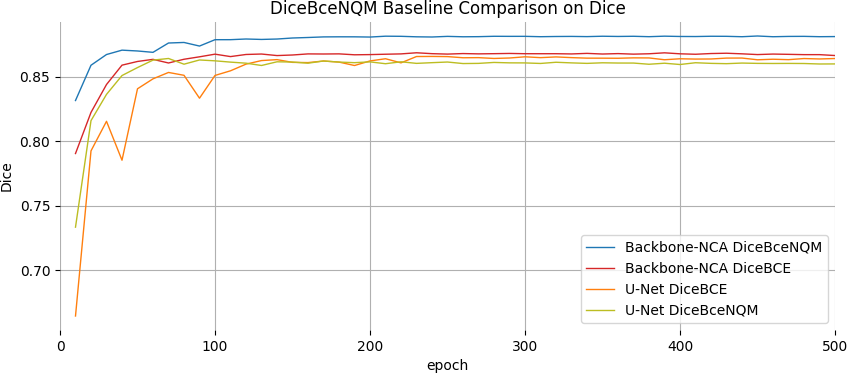
\includegraphics[width=\linewidth]{Graphics/Experiments/2.1_inverted_freeAxes_Loss_DiceLoss()_test_mask0.png}
        \caption{Backbone-NCA trained on DiceBceNQM (blue). For comparison, as baselines, a Backbone-NCA trained on DiceBCE and two U-Nets are given. The convergence of the Backbone-NCA on DiceBceNQM is quite similar to the Baselines. Therefore, training is stable on this loss regarding the Dice score. The U-Nets have been trained for 1000 epochs in total, but the Dice does not change any further, even so the train loss does.}
    \label{fig:02.1:DiceBceNQM:Baselines:onDice}
\end{figure}

As we have seen in \autoref{experiments:01.0:Into}, using only the NQM as a loss function cannot work because the reference to the ground truth label is missing, and since the models we use, the Backbone-NCA as well as the Med-NCA, already use a well working loss; the DiceBCE given in \ref{DiceBCE-Loss} is close to it, to go from there. In this way, we have developed a working NQM-loss function, which works as well as the DiceBce in our first tests, just by adding the NQM to the DiceBCE. The DiceBceNQM, as we later used it mainly for our robustness improvement experiments.

Since the NQM can be very large in the initial training cycles, we additionally cropped the NQM to a value of $\in(0,1)$ to relax the weight of the NQM in the total loss. This results in the DiceBceNQM as follows:

\begin{align}
    \text{DiceBceNQM} &:= 1 - \mathrm{Dice} + \mathrm{Bce} {\color{red}+} \mathrm{NQM},\label{eq:02.1:DiceBceNQM}\\           
    \mathrm{NQM}\ &:=\ \min\left(1, \quad \frac{\sum_{s\in SD} (s) +1} {\sum_{m\in\mu} +1}\right), \qquad
    SD = \sqrt{\frac{\sum^N_{i=1}(v_i-\mu)^2}  {N}  \varepsilon}, \qquad
    \mu = \frac{\sum^N_{i=1}v_i}  {N}               \label{eq:02.1:Only_NQM}
\end{align}

As can be seen in \autoref{fig:02.1:DiceBceNQM:Baselines:onDice} (for Dice), \autoref{fig:02.1:DiceBceNQM:Baselines:onTrainLoss} (for train losses), the Backbone-NCA converges on the DiceBceNQM about as well as on the DiceBCE, measured on Dice, or even slightly better (+1.8 points). We also trained two U-Nets, one on the DiceBCE, the other on the DiceBceNQM, as additional baselines. The convergence is approximately similar to the Backbone-NCA trained on DiceBCE. Furthermore \autoref{fig:02.1:DiceBceNQM:Baselines:Segmentations} show segmentations for the final model and baselines. As can be seen by eye the predictions with the DiceBceNQM are as good as with the DiceBCE. Putting all this together, training on this loss is stable and reliable and as least as good as on the DiceBCE alone. Therefor we used it for most of our robustness tests in \autoref{experiments:03.0:Intro}. 

\begin{figure}[h!]
    \vspace{0.5cm}
    \centering
        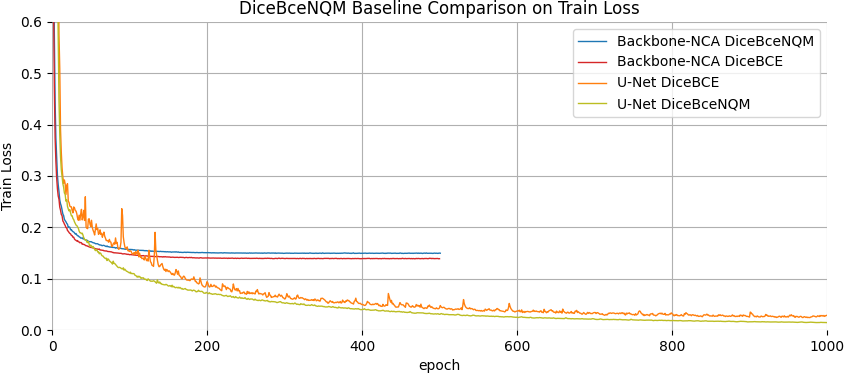
\includegraphics[width=\linewidth]{Graphics/Experiments/2.1_train_loss_freeAxes_Loss_train_0.png}
        \caption{Backbone-NCA trained on DiceBceNQM (blue). For comparison, as baselines, a Backbone-NCA trained on DiceBCE and two U-Nets are given. The convergence of the Backbone-NCA on DiceBceNQM is quite similar to the Baselines. Therefore, training is stable on this loss regarding. The U-Nets have been trained for 1000 epochs in total, Backbone-NCAs only 500 epochs.}
    \label{fig:02.1:DiceBceNQM:Baselines:onTrainLoss}
\end{figure}

\begin{figure}[h!]
    \vspace{0.5cm}
    \centering
        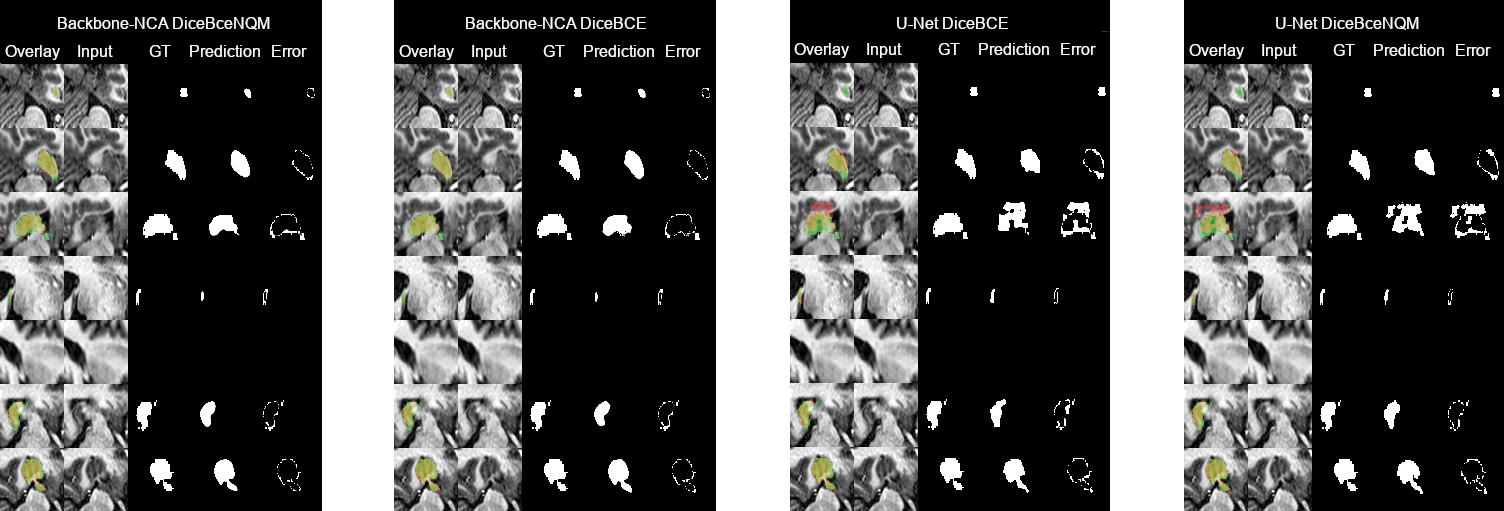
\includegraphics[width=\linewidth]{Graphics/Experiments/2.1_BaselineComparison.png}
        \caption{Backbone-NCA trained on DiceBceNQM (left). For comparison, as baselines, a Backbone-NCA trained on DiceBCE and two U-Nets are given. For each model the same image volumes (inputs) are given. With ground truth labels (GT), predictions, and errors. The overlay shows the input image with false positive (red), true positive (yellow), and  false negative (green). All for the final models after 500 epochs for Backbone-NCAs and 1000 epochs for U-Nets. First and foremost the predictions with the DiceBceNQM for the Backbone-NCA are at least as good as with the DiceBCE. Therefor training on the DiceBceNQM is stable. Even so some segmentations by the U-Nets look worse, then by the Backbone-NCAs, the Dice is is quite similar (\autoref{fig:02.1:DiceBceNQM:Baselines:onDice}).}
    \label{fig:02.1:DiceBceNQM:Baselines:Segmentations}
\end{figure}


We also tested different stacksizes and alpha-values, like in \autoref{experiments:03.1.0:backbone_hippo:intro} and here even in more configurations then there, but since, they did not show any effect here (but there), they are introduced in \autoref{experiments:03.1.0:backbone_hippo:intro}.                 % subsection
\subsection{Further Mixed Dice-Bce-NQM Losses}
\label{experiments:02.2:FurtherDice-Bce-NQMLosses}
%%%% Intro %%%% 
After and before we had our first successes with the DiceBceNQM loss (\autoref{experiments:02.1:diceBce+NQM}), in the sense that we were able to develop a loss that was no worse than the DiceBCE alone, we tried several other implementations to incorporate the NQM into the DiceBCE loss. However, they were all worse than the DiceBceNQM, or at least no better. However, since the DiceBceNQM was the simplest of the equally good losses, we decided, in the spirit of Occam's razor, to start the robustness experiments (\autoref{experiments:03.0:Intro}) with the DiceBceNQM. The more promising of these were tested again in \autoref{experiments:03.1.x:FurtherNQMLosses}, but showed no improvement over the DiceBceNQM in the experiments here without robustness testing, and were judged here to be more computationally expensive or were developed later and are therefore not yet available. These losses are presented in \autoref{experiments:03.1.x:FurtherNQMLosses} and are omitted here to avoid duplication, even though they are clearly better. For the sake of completeness, we list here the loss functions that are worth mentioning, even if they did not make it to the next round.

For the case of the additive DiceBceNQM (\autoref{experiments:02.1:diceBce+NQM}), we also tested whether taking only Dice+NQM or only Bce+NQM had a positive effect, but as suspected, this was not the case.


%%%% Offen / TODO %%%%
\iffalse
... hier stimmte irgendwas nicht ...
... diceBceMasks (Bce with no reduction) was used and the nqm was put in as weight, before the mean was build ... therefore the nqm was calculated pixelwise ... but did not work
\begin{align}
    \mathrm{DiceBceMaskNQM}     &= \mathrm{DiceLoss} + \mathrm{mean} (NQM_mask \cdot \mathrm{BCE})\\
    \mathrm{BCE}(x,y)           &=  -[y_n \cdot \log x_n + (1-y_n) \cdot \log (1-x_n)]\\
    \mathrm{DiceLoss}           &= 1 - \frac{2 \cdot {\sum^D(y \cdot f_\theta(x))}}
                                            {\sum^D(f_\theta(x)) + \sum^D(f_\theta(x))}
\end{align}
... diceBce SD
... Bce weighted with NQM


\fi
%%%% Inputs %%%%
\paragraph{NQM Loss on Pretrained Model}
\label{experiments:02.2.1:Only_NQM_Pretrained}
As a first "naive" test to circumvent the problems in \autoref{experiments:01.1:Only_NQM}, before we developed the DiceBceNQM (\autoref{experiments:02.1:diceBce+NQM}), we have taken a pretrained models with the DiceBCE.

\begin{align}
    \ell(y_i, f_\theta(x_i))\ :=
      \begin{cases}
        \mathrm{DiceBCE} & \text{if epoch {\color{red}$\leq n$}}\\
        \mathrm{NQM} & \text{else}\\
      \end{cases}
\end{align}

Regardless of how long the model was pretrained, as soon as the loss was switched to the NQM the loss dropped enormously quickly towards zero, for the same reason, as for the NQM alone. The output looks the same as in \autoref{fig:exp.01.1:DiceBce_vs_NQM_only} (left).

%%% Alternating
Since it is only a little adjustment form there, we also checked, if this can already be prevented if we alternate between the NQM and DiceBCE. So the loss becomes:

\begin{align}
    \ell(y_i, f_\theta(x_i))\ :=
      \begin{cases}
        \mathrm{NQM} & \text{if epoch {\color{red} mod $x=0$}}\\
        \mathrm{DiceBce} & \text{else}\\
      \end{cases}
\end{align}

However, this attempt suffers from the same problem. For comparison, \autoref{fig:exp.02.1:alternating} shows that already after three epochs on the NQM, the output looks as bad as \autoref{experiments:01.1:Only_NQM} and moreover, already in the very first epoch no useful prediction is left anymore So, for larger $x$ this attempt only takes longer but still converges to the same state, while the epochs with the DiceBCE work in the opposite direction.

\begin{figure}[h!]
    \centering
    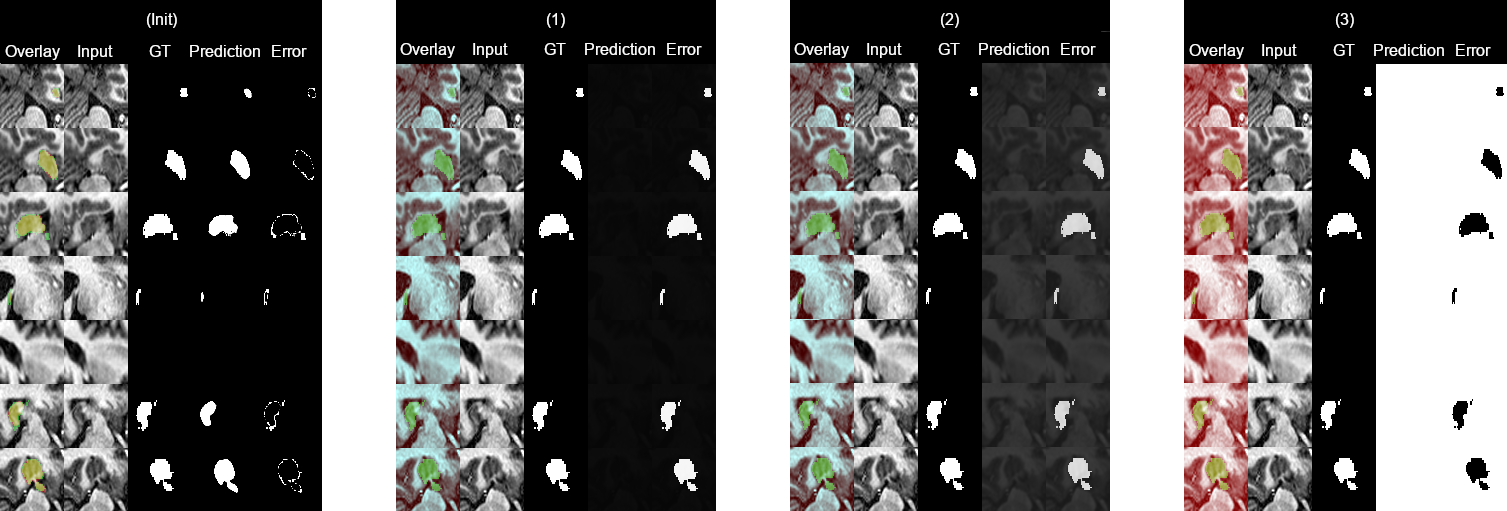
\includegraphics[width=\linewidth]{Graphics/Experiments/4.2.1_Alternating_3epochs_v3.png}
    \caption{Image samples volumes (inputs) with ground truth labels (GT), predictions, and errors. The overlay shows the input image with false positive (red), true positive (yellow), and  false negative (green). From left to right: The initial state, pretrained on DiceBCE (Init), the three very first epochs of training on the NQM.}
    \label{fig:exp.02.1:alternating}
\end{figure}
\paragraph{Multiplicative Dice-Bce-NQM Losses}
\label{experiments:02.2.2:dice+NQM}
To give the NQM more weight in the loss, we also used the NQM as a factor before the DiceBCE. Therefore, we tested the following three implementations of a multiplicative DiceBceNQM loss. However, they all suffered from the same problem as the NQM alone (\autoref{experiments:01.1:Only_NQM}) and the pretrained versions (\autoref{experiments:02.2.1:Only_NQM_Pretrained}). DiceBce*NQM-2 and 3 canceled only the part that has been multiplied with the NQM. Therefore, we tested, with the NQM as defined in \autoref{eq:02.1:Only_NQM}:

\begin{align}
    \text{DiceBce*NQM-1}\ &:=\ {\color{red}\mathrm{NQM}\ \cdot\ }(1 - \mathrm{Dice} + \mathrm{Bce})\\
    \text{DiceBce*NQM-2}\ &:=\ {\color{red}\mathrm{NQM}\ \cdot\ }(1 - \mathrm{Dice}) + \mathrm{Bce}\\
    \text{DiceBce*NQM-3}\ &:=\ 1 - \mathrm{Dice} + {\color{red}\mathrm{NQM}\ \cdot\ }\mathrm{Bce}\\ 
\end{align} % subsection 